\chapter{Model}\label{chap:model}
In order to model networking effects and selfish mining, it is essential to capture network properties in an analytic model. The model can then be used to estimate selfish mining profitability.
\citeauthor{gopalan} have introduced a new blockchain model, which captures network properties.

\paragraph{Gopalan Model}\label{gopalan}
The model of \citeauthor{gopalan} consists of a set of peers $P$ connected through a peer-to-peer network. Peers add blocks to the blockchain through a process called mining. 

The peer-to-peer network is modelled as an undirected Graph $H = (V,E)$.
An edge $(i,j) \in E$ represents communication possibilities between $v_i \in V$ and $v_j \in V$. 
The set of vertices is finite, such that $|V|=N \in \mathbb{N}$.
Vertices are associated with peers, such that $v_i$ represents peer $p_i \in P$.

Additionally, a directed acyclic graph $G_{p_i}(t) = (B_{G_{p_i}}(t),E_{G_{p_i}}(t))$ is associated with each peer $p_i$, at each point in time $t \in \mathbb{R+}$.
The vertex set $B_{G_{p_i}}(t) \subset \mathbb{N}$ represents the blocks known of peer $p_i$ at time $t$. The associated edge set of $E_{G_{p_i}}(t)$ represents references between blocks.
The following holds true for shorter notations:
$B_G(t) = \cup_{i=1}^N B_{G_{p_i}}(t) \texttt{ and } E_G(t) = \cup_{i=1}^N E_{G_{p_i}}(t)$
\textcolor{red}{aber warum eigentlich? macht die zeitabhängigkeit das ganze nicht kaputt?}

Furthermore, the following equations hold for the principle of blockchains:
\begin{equation}
\forall p \in P: G_{p_i}(0) = (\{0\},\emptyset)
\label{genesis}
\end{equation}
\begin{equation}
t_1 < t_2 \rightarrow B_{G_{p_i}}(t_1) \subseteq B_{G_{p_i}}(t_2)
\label{nodegrow}
\end{equation}
\begin{equation}
t_1 < t_2 \rightarrow E_{G_{p_i}}(t_1) \subseteq E_{G_{p_i}}(t_2)
\label{edgegrow}
\end{equation}

Note that in this representation $0$ denotes the genesis block described in equation~\ref{genesis}.

$G_{p_i}(t)$ evolves over time. Blocks arrive over continuous time according to a stationary point process $A$ with intensity $\lambda$. Each block $b \in \mathbb{N}$ arrives at a random peer $p_i$.
This models peer $p_i$ mining block $b$ at time $t$ and that at this time the block is also added to $B_{G_{p_i}}(t)$.

References are added to $E_{G_{p_i}}(t)$ according to policy and depending on $G_{p_i}(t^-)$, where $t^-$ is a moment in time infinitesimally before $t$. $O_i$ denotes the set of outgoing neighbors of block $i$.

The communication is modelled as a marked point process $T_{p_i}$.
Each mark corresponds to another peer $p_j \in P\backslash \{p_i\}$.
In an epoch peer $p_i$ contacts $p_j$ and thus, adds the lowest numbered block of $B_{p_i}(t)\backslash B_{p_j}(t)$ to the set of Vertices $B_{p_j}$. If $B_{p_i}(t)\backslash B_{p_j}(t)$ is not empty, $E_{p_j}$ is also updated accordingly.

The peer-to-peer network dynamics are modelled as a continuous time rumor-spreading process with exogenous arrivals~\citep{gopalan}. Since communication is bound to the process $T_{p_i}$, the block dissemination is bandwidth limited.
Reference selection and thus $O_{p_i}$ is chosen accordant to longest chain policies~\citep{gopalan}.

Let $L_{p_i}(t)$ denote the set of nodes farthest away from the genesis block $0$, known to peer $p_i$ at time $t$.
\begin{equation}
L_{p_i}(t) := \{j \in B_{p_i}(t): d(j,0)\geq d(j',0), \forall j' \in B_{p_i}(t) \}
\label{policy}
\end{equation}

Note that the set $O_{p_i} \cap L_{p_i}(t)$ is non empty. This constructs a simple directed acyclic graph. The Tree Policy~\citep{gopalan} can then be determined as $|O_{p_i}|=1$ and establishes the following relationship:
\begin{equation}
|E_{G_{p_i}}(t)| = |B_{G_{p_i}}(t)| -1
\end{equation}
Every block will have exactly one outgoing reference, according to some deterministic rule~\citep{gopalan}. \citeauthor{gopalan} assume that the block with the lower index number will be chosen.


\paragraph{model extension -- selfish mining inclusion}
The selfish mining attack is described as a peer executing a protocol deviant from honest mining~\citep{eyal}. Therefore a selfish miner can be modelled according to the model described in \ref{gopalan} through altering the reference selection and communication process. The reference selection process is policy driven, and can thus be modified by providing a new selfish policy. 

Peer $SM \in P$ has an associated policy slightly different to \ref{policy}. Note that to follow the Tree Policy~\citep{gopalan}, a deterministic rule has to be established for the case that $|O_{SM} \cap L_{SM}(t)| > 1$.

Assume that $SM$ has the knowledge of the set of blocks mined through him, $M_{SM}(t) \subset B_{G_{SM}}(t)$. $SM$ will set 
\begin{equation}
(L_{SM}(t) \cap M_{SM}(t)) \neq \emptyset \rightarrow L'_{SM}(t) \subset ( L_{SM}(t) \cap M_{SM}(t)) 
\label{smpolicy}
\end{equation}
It then follows that $|L'_{SM}(t)|=1$.
This modified tree policy sets references according to the original selfish mining protocol described by \citeauthor{eyal}.

The second aspect to be modified is the communication process. It will be shown that through modification of the communication process the number of cases, where $|O_{p_i} \cap L_{SM}(t)| > 1$ increases, thus, making \ref{smpolicy} impactful.

Key idea of selfish mining is block withholding. As such the selfish miner not only possesses a blockchain representation of the form $G_{p_i}(t) = (B_{G_{p_i}}(t),E_{G_{p_i}}(t))$, but rather $G_{p_i}(t) = G_{SM_{public}}(t)\subseteq G_{SM_{private}}(t)$, where $G_{SM_{private}}(t)\backslash G_{SM_{public}}(t)$ represents blocks mined but unpublished by the selfish miner.

\begin{figure}
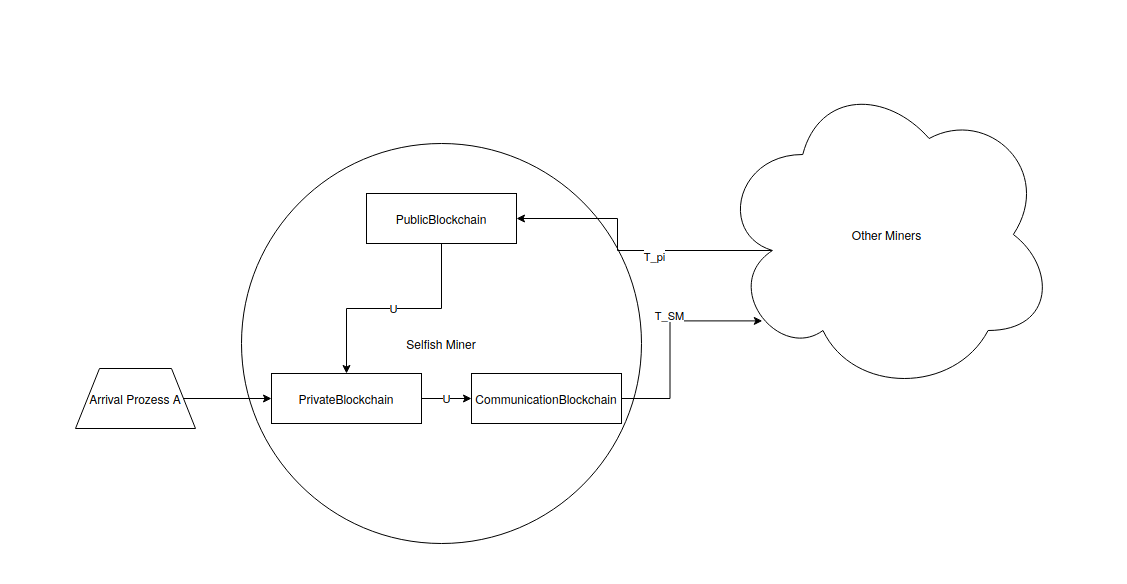
\includegraphics[width=\linewidth]{figures/model_vis1.png}
\caption{\textcolor{red}{keine finale skizze, nochmal überarbeiten etc.}}
\label{fig:model_vis}
\end{figure}

The concept has been visualized in 

$G_{SM_{comm}}(t)$, a third representation, is used to update other peers just as described in \ref{gopalan}. $G_{SM_{private}}(t)$ interacts with $G_{SM_{public}}(t)$ through an instantaneous update process $U$.
The first task of $U$ is to ensure that $G_{SM_{public}}(t)\subseteq G_{SM_{private}}(t)$ holds true, meaning $U$ updates $G_{SM_{private}}(t)$, when new blocks arrive to $G_{SM_{public}}(t)$.

The second task of $U$ is updating $G_{SM_{comm}}(t)$ according to $G_{SM_{private}}(t)$, which is the heart of the selfish mining protocol described by \citep{eyal}.

Let $s$ be the state variable determining selfish mining actions~\citep{eyal}.

Then $s$ can be described as a difference between $G_{SM_{private}}(t)$ and $G_{SM_{public}}(t)$.
\begin{equation}
max\_ dist(G_{p_i}(t)) := d(j,0), j \in L_{p_i}(t)
\end{equation}
\begin{equation}
s(t) := max\_ dist(G_{SM_{private}}(t)) - max\_ dist(G_{SM_{public}}(t))
\end{equation}

Let $t_{inc}$ refer to the set of times, where $s$ increased and analogous $t_{dec}$ refer to the set of times, where $s$ decreased.
Let $f_{-1}(t)$ be a function that outputs the point in time, where s changed the latest before $t$.
$U$ can then be characterized through three kind of update actions. This can be used to model the selfish mining protocol desribed by \citeauthor{eyal}.
\begin{enumerate}
\small
\item Assume $t \in t_{inc}$ and $s(t) \geq 2$, then $U$ updates $G_{SM_{comm}}(t)$, such that $G_{SM_{comm}}(t) = G_{SM_{private}}(t)$.
\item Assume $t \in t_{dec}$ and $s(t) = 0$, then $U$ updates $G_{SM_{comm}}(t)$, such that it includes the subgraph induced by the nodes on the paths between $L'_{SM}(t)$ and ${0}$.
\item Assume $t \in t_{dec}$ and $s(t) = -1$, then $U$ updates $G_{SM_{comm}}(t)$, such that $G_{SM_{public}}(t) \subseteq G_{SM_{comm}}(t)$.
\item Assume $t \in t_{inc}$, $s(t) = 1$, $s(f_{-1}(t)) = 0$, $s(f_{-1}(t)^-) = 1$, then $U$ updates $G_{SM_{comm}}(t)$, such that it includes the subgraph induced by the nodes on the paths between $L'_{SM}(t)$ and ${0}$.
\end{enumerate}

\textcolor{red}{ kann man, darf man $T_{SM}$ modifizieren?}








